
\section{Demonstration}
\label{sec:demo}

We developed a Web interface to allow users to experience our Qsearch system. Figure \ref{fig:gui} shows a screenshot of the top search results for an example quantity query.

%\noindent \textbf{Implementation Details.} // TODO (machine, language, library)



%\noindent \textbf{Input.} Qsearch allow users to type a quantity query as input. 
%% The input question is mapped into Qquery format by a rule-based parser for recognizing answer type and quantity condition; all other tokens (except stopwords) are included in the query context \cite{HoISWC2019}. The parser uses a dictionary of YAGO types and a dictionary of quantity units.
%% An alternative to this rule-based technique would be to apply the same neural extraction method to questions that we have used to extract Qfacts from text. However, the questions are easier to handle, and the rule-based parser works well. 
%To give a better search experience, we show to the users a list of top YAGO types when typing the query, along with the number of relevant entities existing in our database. Figure \ref{fig:type} illustrates an example of this feature.

\noindent \textbf{Input.} Users can provide query in natural language text as input to the system. 
%The query must include one entity type and quantity. 
To give better search experience, we guide users by showing a list of top YAGO types along with the number of relevant entities existing in our database while writing the query. Figure \ref{fig:type} illustrates this feature.

\begin{figure}[t]
\centering
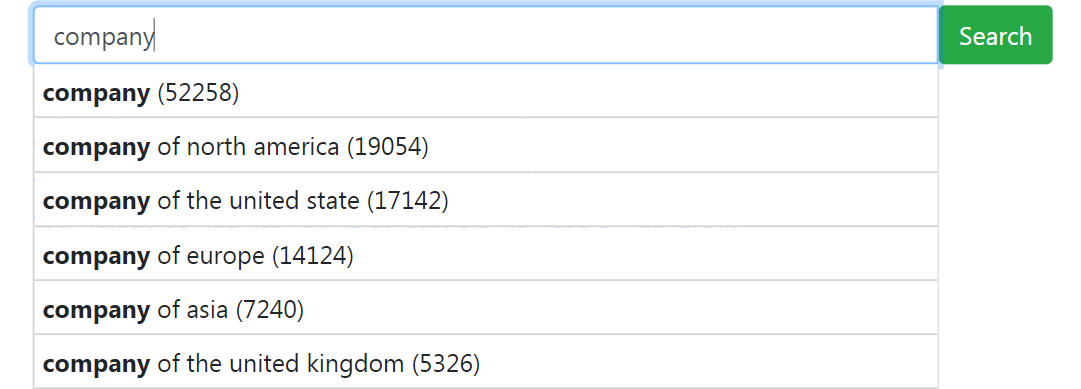
\includegraphics[width=0.5\textwidth]{figures/new/suggest.png}
\caption{Type suggestion in Qsearch.}
\label{fig:type}
\vspace{-1em}
\end{figure}

%\noindent \textbf{Output.} Qsearch processes the input query, looks for relevant entity answers and ranks them based on their distance scores to the query (using either \textit{Kullback-Leibler divergence} or \textit{context embedding distance}).

\noindent \textbf{Output.} Qsearch processes the input query and generates a ranked list of entities relevant to the input query. 
The parsed query, top answers and their entity pages (from Wikipedia) are shown to users, along with the text snippets from where the Qfacts are extracted, and the links to the original web pages (see Figure \ref{fig:gui}). For better experience, we also show the representation images of the entity answers (extracted from the entities' Wikipedia pages) to the users when they hover on the entity links. For each answer, Qsearch highlights the extracted entity, quantity and context cues of the Qfact, and also provides the converted quantity value if its unit is different from the one being asked in the query. In Table \ref{table:sample_q}, we provide some anecdotal examples of user queries and their top answers produced by Qsearch.


%!TEX root = ../main.tex
\begin{table}[t]
	\caption{Sample quantity queries and results from Qsearch.}	
	\small	
	\begin{tabular}{p{.46\textwidth}} \hline
Query \\ \hline
\textbf{Q1:} Skyscrapers with height above 1000 feet\\ 
\textbf{Q2:} Footballers with transfer cost more than 50 million Euros \\  
\textbf{Q3:} Sprinters who ran 100 meter in less than 10 seconds  \\  
%\textbf{Q4:} Companies of Europe having more than 100 thousand employees\\ \bottomrule 
	\end{tabular}
	\small
	\begin{tabular}{l| p{.08\textwidth} p{.30\textwidth}} 
	 \hline
		Query & Result & Corresponding Sentence \\ \hline
		\multirow{2}{*}{Q1}& Empire State Building & 102nd Floor Building: Empire State Building, New York Height: 1,250 feet.\\ 	\cline{2-3}	
		& Mercury City Tower & 	Eleven high-rises have already been built, among them the golden Mercury City Tower, at a height of 339 meters, the tallest skyscraper in Europe.\\ 
		\hline
		\multirow{2}{*}{Q2} & Neymar & The judge says Neymar cost at least 83.3 million euros (\$88 million), while Barcelona insists it paid 57 million euros (then \$74 million). \\ 	\cline{2-3}
		& Raheem Sterling & 	Raheem Sterling became the most expensive English footballer ever on Tuesday after joining Manchester City from Premier League rival Liverpool in a drawn-out move costing 49 million pounds (\$114 million).\\ 
		\hline
		
		\multirow{2}{*}{Q3} & Andre De Grasse & Andre De Grasse, a 20-year-old from Markham, Ont., has run the 100 metre in under 10 seconds three times this year. \\ 	\cline{2-3}
		& Walter Dix & 		Walter Dix, a Florida State sprinter, ran the 100 meter dash in 9.93 seconds, the fastest time in the world this year and the second fastest ever by a collegian.\\ 
		\hline
%		\multirow{2}{*}{Q4}		& Tyco International & 	Based in Bermuda, with headquarters in Exeter, N.H., Tyco has 240,000 employees and makes everything from security systems to syringes.\\ 
%\cline{2-3}

		
% & Volkswagen Group & Volkswagen Group, with its multiple brands, has more than 600,000 employees but the cuts will mainly fall on its 120,000-strong German work force. \\  	
%		\hline
	\end{tabular}	
	\label{table:sample_q}
	\vspace{-1em}
\end{table}


%\noindent \textbf{Text Corpora.} We use a large collections of news articles, compiled from two real world datasets: the \textit{STICS} project \cite{DBLP:conf/sigir/HoffartMW14} with news from 2014 to 2018 (containing 5.84M documents), 
%and the \textit{New York Times} archive
%%\cite{nyt}
% %5843811 + 1765538
%with news from 1986 to 2008 (containing 1.77M documents). These datasets are also used in our earlier work \cite{HoISWC2019}. Moreover, we also integrate a collection of Wikipedia web pages in this demonstration (containing 5.78M documents). In total, our text copora consist of 13.39M documents.
%\noindent \textbf{Explore Qsearch.} Our demonstration system answers quantity queries based on information from three large collections of text documents. Two real world news corpora are used: the \textit{STICS} project \cite{DBLP:conf/sigir/HoffartMW14} (containing 5.84M documents) and the \textit{New York Times} archive (containing 1.77M documents)
\noindent \textbf{Exploration of underlying data sources.} Qsearch answers quantity queries based on information from three large collections of text documents - two real-world news corpora, the \textit{STICS} project \cite{DBLP:conf/sigir/HoffartMW14} (containing 5.84M documents) and the \textit{New York Times} archive \cite{nyt} (containing 1.77M documents), and a collection of web pages from the English Wikipedia\footnote{\url{https://meta.wikimedia.org/wiki/Data\_dump\_torrents\#English\_Wikipedia}}(containing 5.78M documents). In total, our text data consists of 13.39M documents. By default, Qsearch uses all three collections to generate answers. However, we allow users to change this setting (see Figure \ref{fig:settings}) in order to narrow down their search on specific text collections. As the characteristic of news articles is quite different from Wikipedia articles, using both types of text collections as underlying input data allows Qsearch to answer a wide range of quantity queries. For example, information about finance or sport domain can be found all over the news articles and also in Wikipedia, but answers for queries on geological objects (e.g., glaciers with length more than 100 km) are mainly covered only by Wikipedia articles. 
%; these two are also used in our earlier work \cite{HoISWC2019}. Moreover, we also integrate a collection of web pages from English Wikipedia\footnote{\url{https://meta.wikimedia.org/wiki/Data\_dump\_torrents\#English\_Wikipedia}} in this demonstration (containing 5.78M documents). In total, our text data consists of 13.39M documents. 

\noindent \textbf{Exploration of answer generation methods.} Qsearch employs different ranking models as mentioned in Section~\ref{sec:system_overview} to rank the entity answers and shows top confident results to the users. 
In the default configuration, Qsearch uses the \textit{context embedding distance (ced)} as the ranking model, with the penalty factor $\alpha = 3$ (as in \cite{HoISWC2019}), and shows top 20 answers. 
%Qsearch looks for the results in the text documents and shows top 20 most confident entity answers to the users. 
\begin{figure}[t]
\centering
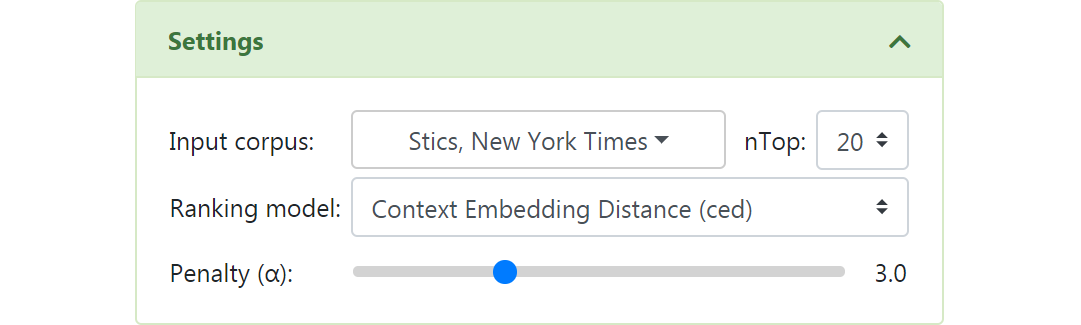
\includegraphics[width=0.5\textwidth]{figures/new/settings.png}
\caption{Qsearch options.}
\label{fig:settings}
\vspace{-1em}
\end{figure}
We provide a flexible interaction to the system by allowing users to modify these search settings (as shown in Figure \ref{fig:settings}) to explore the answer generation methods. 
Here, users can adjust the number of retrieved results (10, 20, 30, 40 or 50) or change the underlying ranking model (\textit{context embedding distance} or \textit{KL-divergence}) and its parameter. Additionally, Qsearch provides further exploration with a secondary ranking criterion, where top retrieved answers can be re-ranked either by quantity value (after normalization), or by entity prominence (based on view count of entities' Wiki pages).
This secondary ranking criterion can be set using \textit{``Sort by''} button in Figure \ref{fig:gui}.
% We provide two different secondary ranking criteria:
% to re-rank the retrieved top entity answers; 





